\begin{figure}[pt]
\centering
\small
\fontfamily{pag}\selectfont
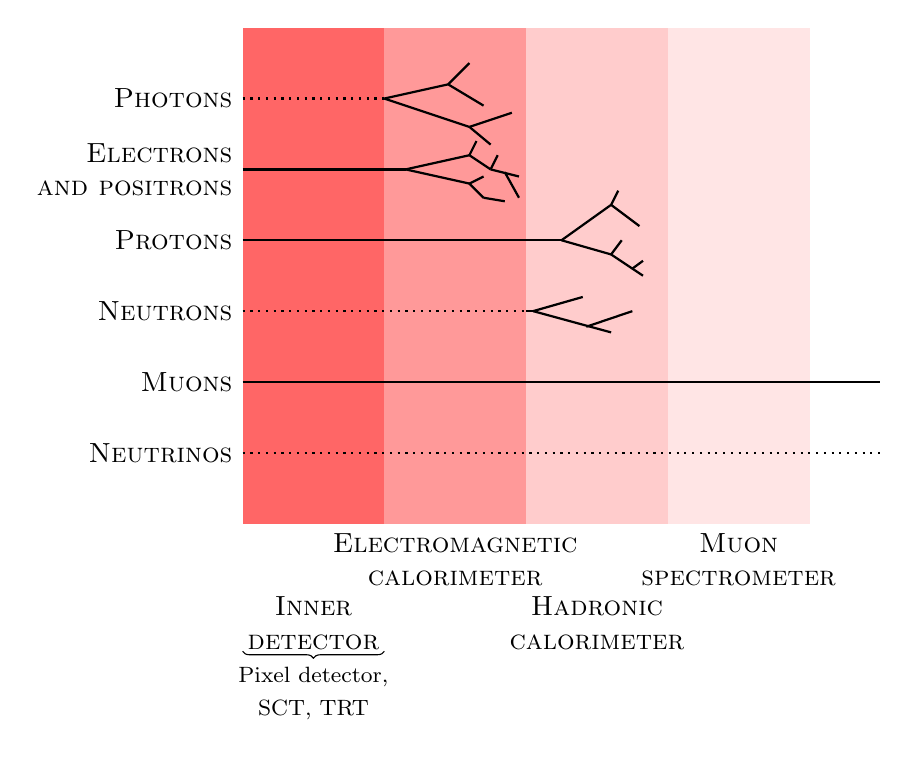
\begin{tikzpicture}[scale=0.9]
	\draw[draw=none,fill=red!60!white] (0,0) rectangle +(2,7);
	\draw[draw=none,fill=red!40!white] (2,0) rectangle +(2,7);
	\draw[draw=none,fill=red!20!white] (4,0) rectangle +(2,7);
	\draw[draw=none,fill=red!10!white] (6,0) rectangle +(2,7);
	
	\draw[thick,dotted] node[left] at (0,6) {\scshape Photons};
		\draw[dotted,thick] (0,6)--(2,6);
		\draw[thick] (2,6)--(2.9,6.2);
			\draw[thick] (2.9,6.2)--(3.2,6.5);
			\draw[thick] (2.9,6.2)--(3.4,5.9);
		\draw[thick] (2,6)--(3.2,5.6);
			\draw[thick] (3.2,5.6)--(3.5,5.35);
			\draw[thick] (3.2,5.6)--(3.8,5.8);
	\draw[thick,dotted] node[left,align=right] at (0,5) {\textsc {Electrons}\\ \textsc{and positrons}} ;
		\draw[thick] (0,5)--(2.3,5);
			\draw[thick] (2.3,5)--(3.2,5.2);
				\draw[thick] (3.2,5.2)--(3.3,5.4);
				\draw[thick] (3.2,5.2)--(3.5,5);
					\draw[thick](3.5,5)--(3.6,5.2);
					\draw[thick](3.5,5)--(3.9,4.9);
						\draw[thick](3.7,4.96)--(3.9,4.6);
			\draw[thick] (2.3,5)--(3.2,4.8);
				\draw[thick] (3.2,4.8) --(3.4,4.9);
				\draw[thick] (3.2,4.8) --(3.4,4.6);
					\draw[thick] (3.4,4.6) -- (3.7,4.55);
	
	\draw[thick,dotted] node[left,align=right] at (0,4) {\textsc{Protons}};
		\draw[thick] (0,4)--(4.5,4);
			\draw[thick] (4.5,4) -- (5.2,4.5);
				\draw[thick] (5.2,4.5)--(5.3,4.7);
				\draw[thick] (5.2,4.5)--(5.6,4.2);
			\draw[thick] (4.5,4) -- (5.2,3.8);
				\draw[thick] (5.2,3.8) -- (5.35,4);
				\draw[thick] (5.2,3.8) -- (5.5,3.6);
					\draw[thick] (5.5,3.6) -- (5.65,3.71);
					\draw[thick] (5.5,3.6) -- (5.65,3.5);
	\draw[thick,dashed] node[left] at (0,3) {\scshape Neutrons};
		\draw[thick,dotted] (0,3)--(4,3);
		\draw[thick] (4,3)--(4.1,3);
			\draw[thick] (4.1,3)--(4.8,3.2);
			\draw[thick] (4.1,3)--(5.2,2.7);
				\draw[thick] (4.85,2.78)--(5.5,3);
	
	\draw[thick] node[left] at (0,2) {\scshape Muons} (0,2) -- (9,2);	
	\draw[thick,dotted] node[left] at (0,1) {\scshape Neutrinos} (0,1) -- (9,1);
	
	\node[align=center] at (1,-1.4) {\scshape Inner\\ \scshape detector};
	\node[align=center] at (3,-.5) {\scshape Electromagnetic\\ \scshape calorimeter};
	\node[align=center] at (5,-1.4) {\scshape Hadronic\\ \scshape calorimeter};
	\node[align=center] at (7,-.5) {\scshape Muon\\ \scshape spectrometer};
	\draw [decorate,decoration={brace}] (2,-1.8)--(0,-1.8);
	\node[align=center] at (1,-2.4) {\footnotesize Pixel detector,\\ \footnotesize SCT, TRT};
\end{tikzpicture}
\caption{Particle behavior inside the various parts of the ATLAS detector, dotted lines are invisible to the various detectors.}
\label{fig:behaviour}
\end{figure}